\chapter{Super-Kamiokande Detector Calibration}
\label{chp:superkcalib}

In order to achieve optimal event reconstruction for physics analyses, calibration of the Super-Kamiokande detector is crucial. For example, when conducting Monte Carlo simulations of certain processes in the detector, facets of the experiment such as properties of the water, photomultiplier tube response and the inner detector and outer detector electronics are all calibrated so that input parameters for the Monte Carlo simulations can be obtained. This chapter will concern itself with the inner and outer detector calibration, including photomultiplier tube and electronics calibration, PMT gain calibration, quantum efficiency determination and hit timing and charge information calibration. 

\section{Inner detector calibration}

\subsection{PMT High-voltage setting calibration}

The high-voltage (HV) setting for all photomultiplier tubes need to be adjusted individually so all the PMTs produce the same amount of charge for a certain light intensity recieved by them. Placing a light source which distributes light isotropically in the centre of the inner detetector to achieve this calibration means that there is no position in the detector from which the inner detector PMTs are equidistant, so each PMT will not recieve the same amount of light from the light source. To avoid this problem, a set of 420 pre-calibrated PMTs inside the detector were used, seperated into groups relating to their geometrical distance from the HV calibration light source, which is shown in Figure \ref{fig:hvcalib} for their location with respect to the other photomultiplier tubes.

\begin{figure}
    \centering
    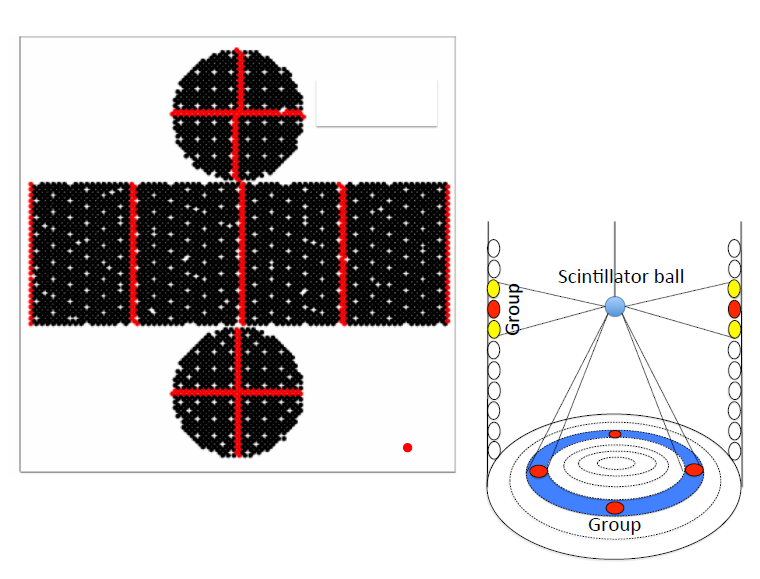
\includegraphics[width=0.7\textwidth]{Figures/hvcalib.png}
\caption{Location of 420 reference PMTs used for HV setting calibration. The red lines in show the placement of these PMTs with repsect to the others (left). The grouping of these PMTs due to their geometry in relation to the light source is also shown (right) }
    \label{fig:hvcalib}
\end{figure}




\subsection{Relative gain calibration}

Understanding the timing information from the hit photomultiplier tubes depends on how well the charge from the hit PMT is calculated. To conceive charge calibration, a quantity called photomultiplier tube ``gain" must be calculated. ``Gain" is the conversion factor from the number of photoelectrons produced by the hit PMT and charge, specifically how much charge one can expect from a single phtotoelectron from the PMT anode. Along with the PMT gain, there are three other quantities which relate to charge calibration: quantum efficiency, collection efficiency and light collection efficiency. 
\newline
The quantum efficiency (QE) is the ratio of the number of photoelectrons produced by the photocathode, to the number of incident photons on the photocathode. The collection efficiency is the fraction of the total number pf photoelectrons produced which are collected by the first dynode in the PMT. The product of the quantum efficiency and the collection efficiency, gives the light collection efficiency.  

 Knowing the gain and light collection efficiency of each PMT in the detector is important in order to accurately measure the output charge from each individual PMT, which is done by first calculating the relative gain difference among all PMTs and then working out the average gain difference over all PMTs in the detector. After this, the variation away from this average gain value can be calculated for each seperate inner detector photomultiplier tube, and the gain value for each can be extracted. 

The relative gain difference is calculated by two measurements using a light source to produce constant-intensity flashes. The first measurement involves using the light source to produce high-intensity flashes so that all photomultiplier tubes in the detctor get a certain number of photons, and the second measurement has the light source produce low-intensity flashes so that only a few PMTs are hit. The first measurement provides an average charge value ($Q_{o b s}(i)$) for each inner detector PMT, while the second measurement gives single photoelectron hits, providing a number of times ($N_{o b s}(i)$) that a single PMT gives a charge which is greater than the PMT threshold value. Equations \ref{eq:gaineq1} and \ref{eq:gaineq2} shows how these two values are calculated from the the high and low intensity flash values ($I$), the acceptance of the PMT(i) ($a(i)$), the QE value of the PMT ($\varepsilon_{q e}$) and the PMT gain $G$. 

\begin{align}
Q_{o b s}(i) \quad \propto \quad I_{high} \times a(i) \times \varepsilon_{q e}(i) \times G(i) \label{eq:gaineq1} \\
N_{o b s}(i) \quad \propto \quad I_{low} \times a(i) \times \varepsilon_{q e}(i) \label{eq:gaineq2}
\end{align}


Therefore, by simply dividing these two values of $Q_{o b s}(i)$ and ($N_{o b s}(i)$) the average gain over all PMTs can be calculated.  Figure \ref{fig:relativegain} shows the spread of the relative gain over all the PMTs. 

\begin{figure}
\centering
    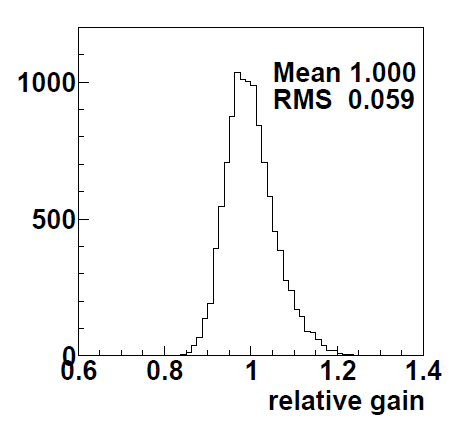
\includegraphics[width=0.7\textwidth]{Figures/relativegain.png}
\caption{Relative gain of PMTs in Super-Kamiokande}
    \label{fig:relativegain}
\end{figure}

\subsection{Absolute gain calibration}

In order to calculate absolute gain, the single photoelectron distrubution needs to be measured, this is because absolute gain relates to the observed charge in the photomultplier tube with the number of photoelectrons produced. A nickel-californium source (shown in Figure \ref{fig:nickel_source}) is used for this measurement due to it releasing gamma rays isotropically, with a total gamma ray cascade energy of 9 MeV. Thermal neutron capture on nickel is used as the gamma ray source, with the neutrons provided by the spontaneous fission of ${ }^{252} \mathrm{Cf}$. This nickel source is placed in the centre of the inner detector and the gamma rays produced are detetced by all the inner detector PMTs. On average the observed number of photoelectrons is 0.004 per event per PMT, meaning that single p.e. hits are observed for more than 99\% of the hits. The observed charge distribution of all the hits from this nickel source is used to give the average charge, which is used as a conversion factor from a charge measurement in picoColoumbs and single photo-electrons. The factor is 2.658 pC per photoelectron (calculated at the beginning of SK-IV) which is then used to extract the single-p.e. distribution, shown in Figure \ref{fig:singlepe}.

\begin{figure}
    \centering
        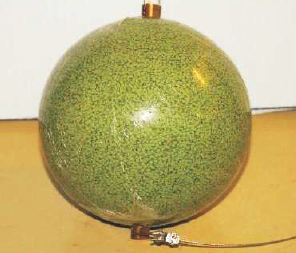
\includegraphics[width=.7\textwidth]{Figures/nickel_source.png}
    \caption{Nickel-californium source used for absolute gain calibration \cite{abe_calibration_2014}}
        \label{fig:nickel_source}
\end{figure}

\begin{figure}
\centering
    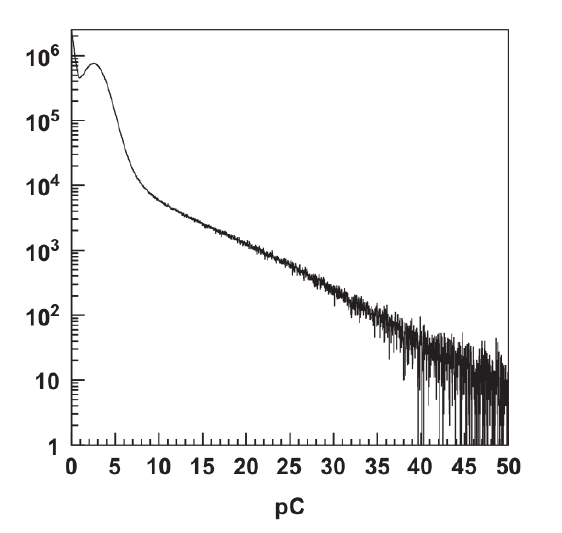
\includegraphics[width=.7\textwidth]{Figures/singlepe.png}
\caption{Single p.e distribution of charge in pC \cite{abe_calibration_2014}}
    \label{fig:singlepe}
\end{figure}
    

\subsection{Relative quantum efficiency measurement}

To measure the relative quantum efficiency, the gamma rays from neutron capture on the nickel source are simulated. Inside this simulation, a common value of QE is used for all the ID PMTs to predict the number of hits for each PMT. Comparing this number of hits to the actual data obtained for each individual PMT by calculating the ratio between them provides us with a value for relative QE for each inner detetor PMT which is then used inside the simulation. 

\subsection{Timing information calibration}
Calibrating the hit timing information of the photomultiplier tubes is essential due to its importance in accurately being able to reconstruct events. Event reconstruction makes use of determining exactly where interaction vertices are and the direction in which particles travel, and to do this the time response needs to be very carefully calibrated. The response time of the PMT also relates to the amount of charge observed: in order for a hit to be registered, the PMT signal must pass the discriminator value of the hit threshold, and the time in which this happens is dependent on the height of the pulse, which is correlated with the observed charge. All thsese factors need to be considered when calibrating hit timing information.
\newline
To aid the timing calibration, a diffuser ball is placed near the centre of the inner detector, into which a nitrogen laser injects pulsed laser light. By varying the intensity of this light, the laser light can be outputted in flashes, and the timing of the laser pulses is monitored using a 2-inch monitor PMT. The schematic of this timing calibration system is shown in Figure \ref{fig:timecalibsystem}.

\begin{figure}
\centering
    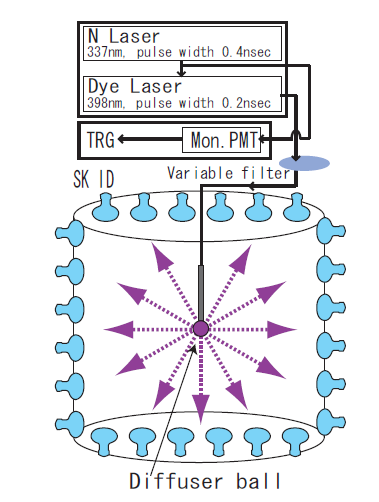
\includegraphics[width=0.7\textwidth]{Figures/timecalibsystem.png}
\caption{Schematic of the timing calibration system, with SK ID PMTs in blue and the diffuser ball in purple. The dye laser shifts the wavelength of the laser light to 398 nm to maximise the quantum efficiency of the PMTs and light absorption.}
    \label{fig:timecalibsystem}
\end{figure}


The value of these laser pulse timings, and the time-of-flight value from the diffuser ball are subtracted from the PMT hit time. Using the observed charge values and these adjusted hit times, ``TQ" (time and charge) distributions can be plotted for each inner detetector PMT. An example TQ distribution is shown for an inner detector PMT (cable number 00010) in Figure \ref{fig:TQdist}, where the vertical axis shows the corrected TOF and laser pulse time corrected PMT hit time, and the horizontal axis shows the observed charge of each hit. Figure taken from \cite{abe_calibration_2014}. 

\begin{figure}
    \centering 
    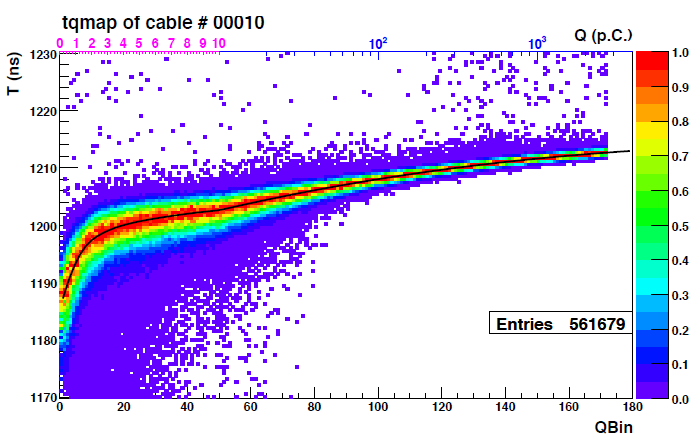
\includegraphics[width=0.7\textwidth]{Figures/TQdist.png}
\caption{Example TQ distribution for an inner detetector PMT}
    \label{fig:TQdist}
\end{figure}


The timing resolution of the PMTs (also known as the transit time spread) is also something that must be calibrated. This is calculated by using the same timing and charge data used to produce the TQ distributions. By correcting all the ID PMT hits by their TQ distributions, these residual timing distributions have an asymmetric Gaussian function fitted to them, from which two values of sigma are extracted: $\sigma_{t}$ and $\sigma_{t'}$. These are the values for the timing resolution for before and after the peak time of this distribution. Equation \ref{eq:sigmat} shows how the asymmetric Gaussian is defined. 

\begin{align}
    f\left(t ; t>T_{\text {peak }}\right) \equiv A_{1} \cdot \exp \left(-\left(t-T_{\text {peak }}\right)^{2} / \sigma_{t}^{2}\right)+B_{1}\\
    f\left(t ; t \leq T_{\text {peak }}\right) \equiv A_{2} \cdot \exp \left(-\left(t-T_{\text {peak }}\right)^{2} / \sigma_{t}^{\prime 2}\right)+B_{2}
\label{eq:sigmat}
\end{align}

Figure \ref{fig:asygausst} shows an example of the residual timing distribution fitted with an asymmetric gaussian for a certain value of binned charge.

\begin{figure}
    \centering
    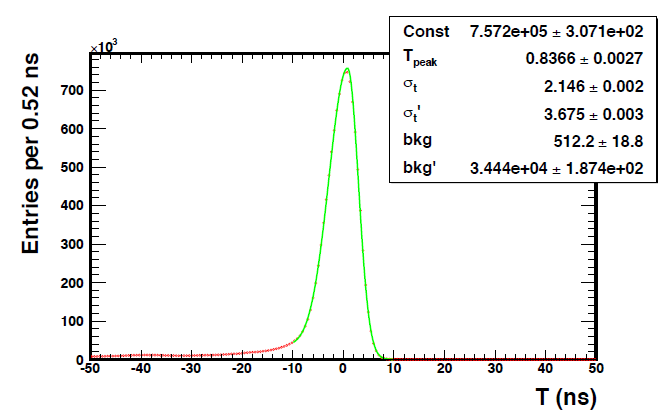
\includegraphics[width=0.7\textwidth]{Figures/asygausst.png}
\caption{Residual timing distribution summed over all the readout channels in charge bin 14 (QBin in \ref{fig:TQdist}.)}
    \label{fig:asygausst}
\end{figure}



Figure \ref{fig:resolutiont} shows timing resolution  plotted as a function of charge for both before and after the peak time of the residual time distribution (red and blue points respectively) for SK-IV TQ calibration data. 

\begin{figure}
    \centering
    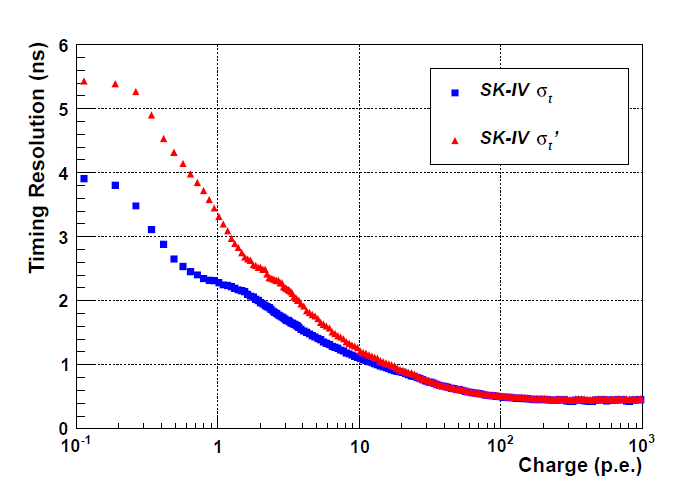
\includegraphics[width=0.7\textwidth]{Figures/resolutiont.png}
\caption{Timing resolution as a function of charge for SK-IV}
    \label{fig:resolutiont}
\end{figure}

\subsection{Measurement of light reflection on the black sheet and the PMTs} 

 For SK-IV, four types of material, corresponding to four different refractive indices are taken into account: water, glass, bialkali, and vacuum. Table \ref{table:refractiveindex} shows the values for each of these materials, $\lambda$ is the wavelength of the light in nm and $n_{real}$ and $n_{img}$ are the real and imaginary parts of the complex refractive index.

Regarding the black sheet used to line the inside of Super-Kamiokande, it can either reflect or absorb Cherenkov photons. The amount of Cherenkov photons dtected is measured by a light injector setup, shown in Figure \ref{fig:blacksheetrefsetup}. For three different incident angles of laser light ($30 \degree$, $45 \degree$ and $60 \degree$) and three different laser light wavelengths (337 nm, 400 nm and 420 nm) the charge from the light scattered off the black sheet was measured. The direct charge (i.e. the same setup without the black sheet present) was also measured, with the total black sheet reflectivity being the ratio between the scattered charge and the direct charge.

\begin{table}
    $$
    \begin{array}{|cc|}
    \hline \text{Material} & \text{Refractive index} \\
    \hline Water & 1.33 \\
    \hline Glass & 1.472+3670/\lambda^{2} \\
    \hline Bi-alkali & n_{real} + i \dot n_{img} \\
    \hline Vacuum & 1.00 \\
    \hline x_{a b s}^{N} & \text { Nucleon absorption probability }  \\
    \hline x_{\pi}^{N} & \text { Nucleon } \pi \text {-production probability }\\
    \hline

    
    \end{array}
    $$
    \caption{Refractive indices of materials inside the Super-K detector.} 
    \label{table:refractiveindex}
    \end{table}
    

\begin{figure}
    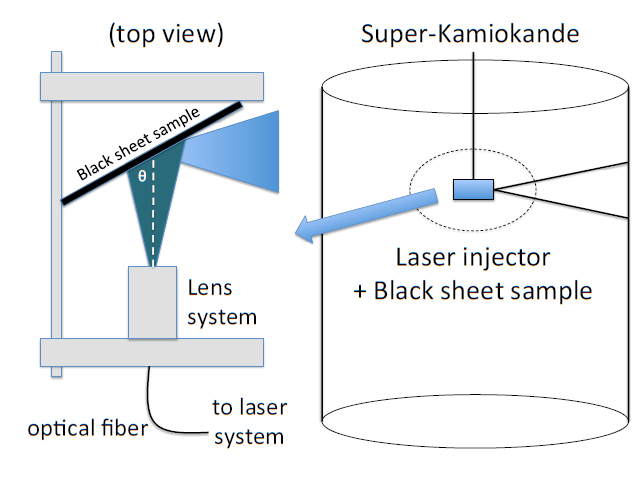
\includegraphics[width=\textwidth]{Figures/blacksheetrefsetup.png}
\caption{Schematic of the laser light reflectivity. Bird's-eye view (left) and setup inside of Super-Kamiokande (right).}
    \label{fig:blacksheetrefsetup}
\end{figure}


\subsubsection{Measurement of absorption and scattering coefficients}

In Super-Kamiokande, the detector medium scatters and absorbs the Cherenkov light, attenuating its wavelength. The amount of light attenuation after the light has travelled distance $l$ is given by $exp(-l/L(\lambda))$. Here $L(\lambda)$ is the attenuation length of the detector medium and is shown by Equation \ref{eq:attenuation_length}, 

\begin{equation}
L(\lambda)=\frac{1}{\alpha_{\text {sym }}(\lambda)+\alpha_{\text {asym }}(\lambda)+\alpha_{a b s}(\lambda)}
\label{eq:attenuation_length}
\end{equation}

In Equation \ref{eq:attenuation_length}, the $\alpha_{\text {sym }}$ parameter is consists of two types of scattering: the symmetric component of Mie scattering and Rayleigh scattering, whereas $\alpha_{\text {asym }}$ only consists of asymmetric Mie scattering.   Figure \ref{fig:rayleigh_mie} shows the difference between these two types of scattering:

\begin{figure}
    \centering
    
\includegraphics[width=0.7\textwidth]{Figures/rayleigh_mie.png}
    \caption{Schematic of the differences between Rayleigh and Mie scattering}
    \label{fig:rayleigh_mie}
\end{figure}

Rayleigh scattering occurs when light is scattered from very small particles, the size of these particles being less than 1/10 of the wavelength of the light. For particles larger than the wavelength of the light being scattered, Mie scattering becomes more dominant, with more asymmetric scattering occuring the larger the particle is (i.e. with a greater forward lobe for larger particles.) As a result of this $\alpha_{\text {sym}}$ has an angular dependance of $1 + cos(\theta)^2$ where $\theta$ is the angle between the incoming and outgoing scattered photon vectors, but $\alpha_{\text {asym}}$ has a $cos\theta$ dependence, only for forward scattering, and an amplitude of zero for backward scattering. The $\alpha_{abs}(\lambda)$ is the amplitude of the light absorption. The method by which these measurements were made is by using a laser system (shown in Figure \ref{fig:laser_system}),  where laser light is injected at several points in the tank, denoted in Figure \ref{fig:laser_system} by the barrel injectors (B1-B5), the previously used old top injector (OT), the new top injector (NT), and an injector on the tank bottom (BT). 

\begin{figure}
    \centering
    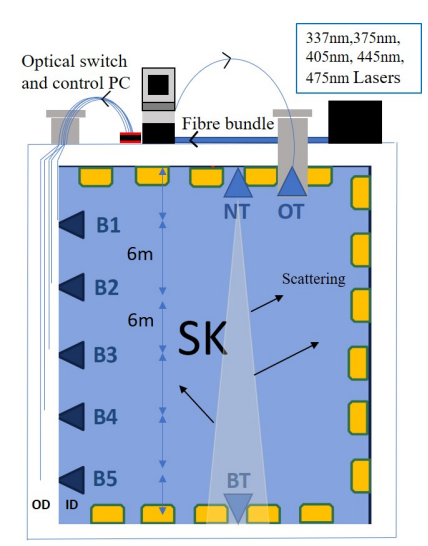
\includegraphics[width=0.7\textwidth]{Figures/laser_system.png}
    \caption{Schematic of the laser system}
    \label{fig:laser_system}
\end{figure}

The absorption and scattering coefficients are measured using data from light injected from the new top (NT) injector. A large set of calibration Monte Carlo are generated using laser generation software and the Super-Kamiokande detector simulation (SKDETSIM). These set of Monte Carlo are generated with different values of absorbtion, symmetric and asymmetric scattering, and their timing distributions are compared to the data from the laser system in order to tune the amount of absorption, symmetric and asymmetric scattering in the calibration Monte Carlo. The way in which the $\alpha_{abs}(\lambda)$, $\alpha_{\text {sym}}$ and $\alpha_{\text {asym}}$ are defined is shown in Equation \ref{eq:P0P8}.

\begin{equation}
\begin{gathered}
\alpha_{a b s}=P_{0} \times \frac{P_{1}}{\lambda^{4}}+C \label{eq:P0P8}\\ 
\alpha_{s y m}=\frac{P_{1}}{\lambda^{4}} \times\left(1+\frac{P_{5}}{\lambda^{2}}\right) \\
\alpha_{a s y}=P_{6} \times\left(1+\frac{P_{7}}{\lambda^{4}} \times\left(\lambda-P_{8}\right)^{2}\right)
\end{gathered}
\end{equation}

The term $C$ in the equation for $\alpha_{abs}(\lambda)$ is based on data from \cite{Pope:97} for laser light with wavelengths greater than 464 nm while Equation \ref{eq:Cformula} is used for wavelengths less than 464 nm. 

\begin{equation}
C=P_{0} \times P_{2} \times(\lambda / 500)^{P_{3}}
\label{eq:Cformula}
\end{equation}

The values of $P_{0}$ to $P_{8}$ in Equations \ref{eq:P0P8} and \ref{eq:Cformula} were taken from fits to laser data taken in April 2009, the water coefficient functions of which are shown in Figure \ref{fig:water_coeff_plot}. 

\begin{figure}
    \centering
    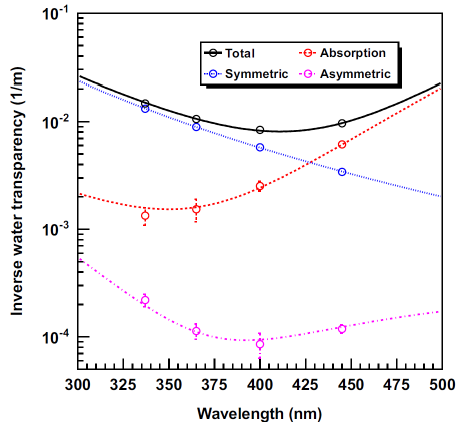
\includegraphics[width=0.7\textwidth]{Figures/water_coeff_plot.png}
    \caption{Plot of water coefficient functions used in Monte Carlo production, showing points for symmetric and asymmetric scattering and absorption.}
    \label{fig:water_coeff_plot}
\end{figure}

As well as the amount of absorption and scattering in the detector, there is also a dependence with respect to z-position in the detector, defined by Equation \ref{eq:tba}.

\begin{equation}
    \alpha_{\text {tba }}=\left(\left\langle N_{\text {top }}\right\rangle-\left\langle N_{\text {bottom }}\right\rangle\right) /\left\langle N_{\text {barrel }}\right\rangle
    \label{eq:tba}   
\end{equation}

Here $\langle N_{\text {top }}\rangle$, $\langle N_{\text {bottom }}\rangle$, $\langle N_{\text {barrel }}\rangle$  are the averaged hit probabilities of the top, bottom and barrel PMTs, where  $\langle N_{\text {top }}\rangle$ is about 5\% less than $\langle N_{\text {bottom }}\rangle$ due to the temperature gradient in the tank. Figure \ref{fig:temperature_grad} shows this dependence, and Equation \ref{eq:temp_grad} shows how this is taken into account for the absorption coefficient $\alpha_{abs}$ by the factor $A(z,t)$:

$$
\begin{aligned}
A(z, t) &=1+z \cdot \beta(t) \quad \text { for } z \geq-11 \mathrm{~m} \label{eq:temp_grad} \\
&=1-11 \cdot \beta(t) \quad \text { for } z \leq-11 \mathrm{~m}
\end{aligned}
$$

where from Figure \ref{fig:temperature_grad}, the value of $A(z,t)$ is constant below $z = -11 m$, and above $z = -11 m$ this value is determined by the z-position in the tank. The relationship between the value of $\beta$ is related to the top-bottom asymmetry parameter $\alpha_{tba}$, and for the April 2009 data $\alpha_{tba}$ and $\beta$ are -4.91\% and 0.01. 


\begin{figure}
    \centering
    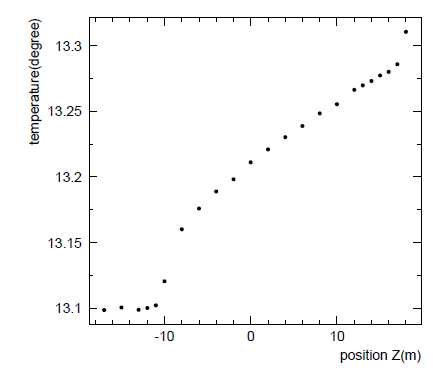
\includegraphics[width=0.7\textwidth]{Figures/temperature_grad.png}
    \caption{Dependence of temperature on vertical position in the Super-Kamiokande ID.}
    \label{fig:temperature_grad}
\end{figure}

Chapter 5 expands upon these measurements by going into detail about the newly developed UK Light Injection system which improves upon the Korean laser system mentioned here used to make water coefficient measurements - it offers much narrower beam profiles which are shone onto the barrel regions, allowing for better analysis of the depth dependence of the water coefficients. 






